\chapwithshorttitle{Concepts, technologies, applications}{Le jumeau numérique : concepts, technologies et application}{Le jumeau numérique : concepts, technologies et application}  
Avant de se pencher sur le traitement des données dans le cadre d'un projet de recherche, il est pertinent d'examiner le concept de jumeau numérique vers lequel ce projet tend. Cette réflexion préliminaire permet de mieux définir ce concept et d'ajuster la gestion des données en conséquence.

    \secwithshorttitle{Historique et définitions}{Historique et définition du jumeau numérique}{Historique et définition du jumeau numérique}

        \subsection{Émergence et évolution d’une technologie prometteuse}

L’idée maîtresse du concept de jumeau numérique remonte aux années 1960. La NASA développe ce qui est aujourd'hui considéré comme l'ancêtre des jumeaux numériques pour ses missions d'exploration spatiale. Lors de la mission Apollo 13, une réplique exacte du vaisseau était présente sur Terre, permettant aux scientifiques de réaliser des tests et de proposer aux astronautes les meilleures solutions lorsque les réservoirs d'oxygène explosèrent en plein vol.\footcite{QuEstceQu2023}\footcite{miskinisMysteriousHistoryDigital2019}

Le concept reste en suspens mais n'est pas réellement exploité. C'est en 1991, lorsque David Gelernter publie Mirror Worlds\footcite{gelernterMirrorWorldsDay1991}, que sont posées les bases conceptuelles de ce qui deviendra plus tard la technologie du jumeau numérique.\footcite{kalilMirrorWorldsBook2024} Gelernter imagine des « mirror worlds », où des systèmes réels comme des villes, des écosystèmes ou des processus industriels sont fidèlement reproduits dans un environnement numérique. Ces mondes numériques reflètent en temps réel l'état de leur homologue physique, offrant ainsi une observation directe des phénomènes à l’échelle micro ou macroscopique. Plus encore, dans ces « mirror worlds », les utilisateurs peuvent interagir avec les systèmes représentés, permettant de comprendre les interactions entre les différents composants. Ces mondes miroirs offriraient une surveillance continue et une gestion proactive des systèmes, permettant d’anticiper les problèmes, d’optimiser les performances, et de prendre des décisions éclairées basées sur des données en temps réel. Gelernter envisageait déjà des applications dans divers domaines, tels que la gestion urbaine, la médecine, l'éducation et les entreprises.\footcite{zadehDigitalTwinMight2024}  Il est néanmoins trop visionnaire pour son époque, alors qu'Internet en est encore à ses débuts. Bien que sa technologie soit saluée par le New York Times, elle reste largement ignorée.\footcite{lehmann-hauptBooksTimesMirror1991}\\

Son idée semble être délaissée. Ce n'est que sept ans plus tard que la dénomination « digital twin » apparaît pour la première fois en 1998, alors qu'elle est utilisée pour désigner une copie numérique de la voix de l'acteur Alan Alda dans le projet intitulé Alan Alda meets Alan Alda 2.0. Ce projet visait à montrer l’acteur en train d’interagir avec une version virtuelle de lui-même,  afin de mettre en avant la façon dont les doublons numériques pouvaient être utilisés dans les médias et le monde du divertissement.\footcite{miskinisMysteriousHistoryDigital2019}\footcite{onceaDigitalTwinsApollo2024} Sans pour autant atteindre l'idée d'un monde virtuel numérique double, le principe de jumeau continue de séduire.\\

C'est en 2002 qu'un nouveau pas est franchi. Michael Grieves, professeur à l'université du Michigan, réalise une présentation. Son but est de rendre les usines et leur fonctionnement plus efficaces, et selon lui, la clé réside dans la création d’une réplique virtuelle parfaitement fidèle de chaque élément physique. Machines, chariots élévateurs, et même travailleurs, tout pourrait être analysé sur un écran d'ordinateur. Ce modèle virtuel serait alimenté en continu par un flux de données, se mettant à jour en temps réel pour refléter avec précision l’usine. Il décrit alors toutes les caractéristiques d’un jumeau numérique moderne : un espace réel, un espace virtuel, la diffusion des données et l’interaction entre les deux types d’éléments.\\

Il faut de nouveau attendre quasiment une décennie pour que la définition du jumeau numérique gagne en précision. En 2010, John Vickers introduit le terme « jumeau numérique » dans un rapport de feuille de route de la NASA intitulé  Technology Area 12 : Materials, Structures, Mechanical Systems, and Manufacturing Road Map (domaine technologique 12 : matériaux, structures, systèmes mécaniques et fabrication). Cette fois-ci, le terme est associé à l'idée qu'on lui donne habituellement. La technologie est définie comme une représentation virtuelle d'un objet ou d'un processus, qui permet de simuler et d'analyser le comportement et les performances de l'objet ou du processus réel. Selon ce rapport, le concept de jumeau numérique se compose de trois parties distinctes : l'objet ou le processus physique et son environnement physique, la représentation numérique de l'objet ou du processus, et le canal de communication entre les représentations physique et virtuelle. Les connexions entre la version physique et la version numérique incluent des flux d'informations et de données, y compris des flux de capteurs physiques entre les objets et environnements physiques et virtuels\footcite{JumeauxNumeriquesGuide}. \\

Avec l'utilisation de plus en plus aisée d'Internet, qui permet l'échange des données en temps réel, et l'évolution de la technologie IoT (Internet of Things), qui désigne les dispositifs connectés qui relient les éléments physiques à leur représentation numérique\footcite{thermosJumeauNumeriqueConcept2024}, l'utilisation des jumeaux numériques devient de plus en plus attractive. C’est ainsi que le concept fleurit très largement dans le courant des années 2020. Un article de 2022 intitulé « Digital Twins: Potentials, Ethical Issues, and Limitations » va même jusqu'à constater que « créer des jumeaux numériques à propos de tout devient une idée attractive »\footcite{helbingDigitalTwinsPotentials2022}. Enfin, le World Economic Forum labellise en 2024 le jumeau numérique comme faisant partie de la « quatrième révolution industrielle », l’inscrivant définitivement au panthéon des nouvelles technologies révolutionnaires.\footcite{batagliaWhyTeamingIndustry2024}.\\

Il est intéressant de noter qu'au cours du développement du jumeau numérique dans l'histoire, trois grandes périodes tendent ainsi à se dégager, périodes où un jumeau numérique ne voulait pas forcément faire référence à une même technologie. Des années 60 jusqu’en 2002, un jumeau numérique est une représentation numérique d’d'un élément concret alimenté par des données pour le rendre aussi réaliste que possible. De 2003 à 2014, le concept s'affine pour inclure des simulations basées sur les résultats de mesures collectées via des capteurs afin de disposer de données à tout instant. Depuis 2015, un jumeau numérique désigne un objet physique connecté en permanence au virtuel, avec une interaction bidirectionnelle : l'objet physique influence l'objet numérique, et vice-versa.\footcite{grievesJumeauxNumeriquesPresentation2019}

 \subsection{La définition du jumeau numérique de nos jours}

    \subsubsection{Définition}

Avant de présenter ce qu'est un jumeau numérique, il convient de préciser que les sources disponibles à ce sujet sont assez rares. Il s'agit en effet d'un sujet niche, dont la définition technique assez complexe semble vouée au changement. En outre, la plupart des présentations techniques des jumeaux numériques se trouvent sur des sites d'entreprises qui offrent leurs services pour en construire, ou sur des blogs intéressés par les évolutions numériques offertes par la technologie, dont les définitions peuvent varier. Les informations qui y sont exposées visent donc à présenter ce qu'est un jumeau numérique dans les grandes lignes, les capacités qu'il offre, mais parlent rarement d'une définition consensuelle. Le jumeau numérique est avant tout considéré comme un outil exploité par le secteur industriel, et commence seulement à gagner en intérêt pour le domaine patrimonial. Par conséquent, si cette technologie a pu faire l'objet de recherches scientifiques, elle est très largement abordée sous un point de vue scientifique et technique, et quasiment jamais patrimonial. Seuls quelques articles commencent à fleurir à ce sujet à partir des années 2010 - 2020, mais ces derniers restent rares.\\

Il est donc ardu de définir précisément ce qu’est un jumeau numérique. La plupart des articles qui tentent d’en fournir une définition se contentent d’énoncer les différentes fonctionnalités qu’il peut offrir\footcite{MiroirMiroirJumeau2021}. Néanmoins, le point principal qui revient systématiquement laisse entendre qu’un jumeau numérique cherche à reproduire tout élément, qu’il s’agisse d’un système, d’un processus, ou d’un objet qui nécessite d’être dupliqué afin d’être étudié.\footcite{miskinisComparingInternetThings2018}. La plupart des définitions proposées convergent vers les mêmes concepts fondamentaux : un modèle physique existant dans ce qui est appelé le « monde réel », un modèle numérique, une interaction entre les deux, et la transmission des données.\\

En outre, aucune définition consensuelle n’a encore émergé au sein de la communauté scientifique. Ce n’est qu’en 2023, que le Digital Twin Consortium propose une définition formelle. Créé en mai 2020, le Digital Twin Consortium (ou DTC) est une organisation mondiale dédiée à la promotion et au développement de cette technologie\footcite{DigitalTwinConsortium}. En collaboration avec l'industrie, le gouvernement et le milieu académique, il cherche à devenir l'autorité en matière de jumeaux numériques en le définissant, en comblant les lacunes technologiques et en publiant des normes, des architectures et des avis. L'objectif est de standardiser la technologie des jumeaux numériques pour qu'elle puisse être utilisée efficacement dans divers secteurs.  Sa définition est la suivante :\\

\begin{quote}« A digital twin is a virtual representation of real-world entities and processes, synchronized at a specified frequency and fidelity.
\begin{itemize}
\item Digital twin systems transform business by accelerating holistic understanding, optimal decision-making, and effective action.
\item Digital twins use real-time and historical data to represent the past and present and simulate predicted futures.
\item Digital twins are motivated by outcomes, tailored to use cases, powered by integration, built on data, guided by domain knowledge, and implemented in IT/OT systems. »\footcite{DefinitionDigitalTwin}
\end{itemize}
\end{quote}

D'après cette définition, un jumeau numérique est une « représentation virtuelle d’entités et de processus du monde réel, synchronisée à une fréquence et une précision données ». Cette définition large, est secondée ici par les fonctionnalités offertes par un jumeau numérique, à savoir la possibilité d’accélérer la compréhension globale d’un système et d’optimiser la prise de décision.\\ 

Le deuxième point soulève une particularité intéressante : pour exister, un jumeau numérique se base sur plusieurs types de données, à savoir des données déjà produites et des données en temps réel. C'est ce qui rend la technologie fascinante : un jumeau numérique est capable de représenter à la fois le passé d’un objet, mais aussi son état actuel et son état à venir. Par exemple, le jumeau numérique d’un avion représenterait non seulement les vols effectués par le passé, l’état de ses moteurs et de son fuselage, mais aussi l’état de ses pièces dans un certain nombre d’années en fonction des données récoltées. Cela implique que l'élément réel soit équipé de capteurs qui permettent au jumeau numérique de récolter ses données et de suivre en temps réel son état tout en évoluant avec lui\footcite{gladieuxJumeauNumeriqueAeronautique2019}.\\ 

Enfin, le dernier volet de cette définition vient rappeler qu’un jumeau numérique n’est pas orienté vers la simple représentation d’un objet ou d’un processus (ce qu'une modélisation pourrait faire), mais davantage vers les résultats produits grâce aux données récoltées et aux analyses effectuées. Il agrège les connaissances disponibles, les données et les simulations relatives au système en question grâce à des capteurs notamment, offrant une analyse approfondie et une anticipation des comportements futurs en s'adaptant aux données en temps réel provenant de l'actif physique\footcite{bealJumeauNumeriqueRealite}\footcite{QuEstceQu2023}.\\

Cette définition met ainsi en avant le type de données qui constituent un jumeau numérique, et qu'il sera intéressant de repérer lors de la gestion des données du projet C-ADER : 
\begin{itemize}
    \item \textbf{Les données actuelles}, c’est-à-dire des données en temps réel provenant des capteurs de l’équipement, des sorties des plateformes et systèmes de fabrication, ainsi que des systèmes de la chaîne de distribution. On pense par exemple aux données de la plateforme « Virtual singapor », qui est sans cesse alimentée par des informations collectées visant à mesurer la qualité de l’air et la température. Dans le cadre du projet C-ACER, il s’agira davantage des données d’analyses effectuées sur les avions du projet, même s’il s’agit plutôt dans la globalité de relevés concernant un instant T, et non pas de relevés en continu. 
    \item \textbf{Les données historiques}, qui comprennent les performances passées des machines, des processus et des systèmes, ou les données retraçant la vie de l’objet réel modélisé. C’est par exemple les données de maintenance des flottes de l’armée de l’air et de la marine nationale, collectées par Dassault aviation et mises dans 3DExperience pour venir alimenter les JN de chaque appareil. Pour C-ADER, on trouverait l’équivalent dans la documentations et les archives relatives à des incidents techniques ou à des réparations d’avions susceptibles de renseigner sur l’état des appareils ; il pourrait également être question de documents relatant les historiques de vols, ou bien plus concrètement les plans et les documents relatifs au système technique de l’appareil.
    \item \textbf{Les Données prédictives} produites par le jumeau numérique lui-même. Issues de l'apprentissage automatique, elles projettent les performances et les comportements attendus. Ce type de données sera absent des jumeaux numériques prévus dans le cadre du programme C-ADER\footcite{rebecchiQuEstceQue2021}.\\ 
\end{itemize}

À la fois outil centralisateur de données, planificateur, ces spécificités font du jumeau numérique un outil qui permet d'accéder à toutes les informations sur l'objet ou le processus représenté sans avoir besoin de l'avoir physiquement à disposition. 

        \subsubsection{Les principes garants de l'efficacité d'un jumeau numérique}

Un jumeau numérique doit respecter plusieurs principes au commencement de sa conception, qui sont essentiels pour garantir l’efficacité de l’outil et qu'il est nécessaire de connaître avant de se pencher sur les types de données à traiter.\\

\begin{enumerate}
    \item Conception Simultanée : Ce principe consiste à développer le modèle numérique et le système physique en même temps. Cette approche assure une synchronisation continue entre le jumeau numérique et son équivalent physique, permettant des ajustements en temps réel et une meilleure intégration des modifications. Par exemple, si on construit un nouvel avion, on crée en parallèle une version numérique qui évolue avec l’avion réel. Cela permet de s'assurer que toutes les modifications apportées à l'avion réel sont également mises à jour dans la version numérique, et vice-versa. Cela permet de détecter et de corriger rapidement des problèmes potentiels.\\
    \item Représentativité : Le jumeau numérique doit représenter fidèlement le système dans son ensemble et reproduire son comportement dans diverses conditions. La représentativité comprend deux sous-critères :
    \begin{itemize}
        \item Expressivité : Capacité à décrire divers phénomènes et scénarios possibles. Cela signifie que le modèle doit être suffisamment détaillé et flexible pour simuler une large gamme de situations, allant des conditions normales aux événements exceptionnels. Par exemple, il doit pouvoir montrer comment l’avion se comporte en vol, lors de l’atterrissage ou dans des conditions météorologiques extrêmes.\\
        \item Précision : Écart minimal entre les résultats simulés et les mesures réelles. Une haute précision assure que les simulations fournies par le jumeau numérique sont fiables et peuvent être utilisées pour des prévisions et des décisions critiques. Par exemple, si l’avion réel consomme 5 litres de carburant par minute en vol, le jumeau numérique doit montrer la même consommation.\\
    \end{itemize}
    \item Interopérabilité : Le jumeau numérique doit pouvoir se connecter et fonctionner avec d'autres applications, jumeaux numériques, ou capteurs physiques. Cette capacité garantit une intégration fluide avec les systèmes existants et futurs, permettant une communication et un échange de données efficaces entre différents composants et plateformes.\\
    \item Présence : Ce critère évalue la capacité du jumeau numérique à permettre à un humain de percevoir et d'interagir avec le système. La réalité virtuelle joue un rôle crucial en offrant une immersion sensorielle dans un environnement simulé. Les utilisateurs peuvent interagir avec le jumeau numérique via divers contrôles tels que la voix, les manettes ou la capture de mouvements, améliorant ainsi l'expérience utilisateur et l'efficacité des formations et des simulations.\\
    \item Explicabilité : Le jumeau numérique doit être transparent et facile à comprendre. Cela signifie qu'il doit être possible d'expliquer comment il fonctionne et pourquoi il donne certains résultats. Cela implique une transparence totale dans les opérations et les processus, facilitant la recherche de solutions en cas de dysfonctionnements et l'optimisation des performances. Par exemple, si le jumeau numérique montre une défaillance dans une pièce de l’avion, il doit être possible de retracer les données et les simulations pour comprendre pourquoi cette défaillance est prévue et comment elle peut être corrigée.\\
    \item Autonomie : Le jumeau numérique doit reproduire fidèlement le comportement du système physique et s'adapter à un large éventail de conditions pour permettre au jumeau numérique d'anticiper et de réagir à des situations exceptionnelles avant qu'elles ne se produisent sur le système physique. Cela inclut la capacité à prendre des décisions basées sur des analyses prédictives et à effectuer des ajustements autonomes pour prévenir des pannes ou optimiser les performances. Par exemple, il doit pouvoir surveiller en continu l’état de l’avion et déclencher des alertes ou des actions correctives sans intervention humaine si un problème est détecté. Cela permet de réagir rapidement aux situations imprévues et de minimiser les risques.\footcite{bealJumeauNumeriqueRealite}
\end{enumerate}

Ces éléments devront ainsi être traités avec considération lors du traitement et de la structuration des données du projet C-ADER lors de leur modélisation.

    \secwithshorttitle{Caractéristiques et potentiels}{Caractéristiques et potentiel des jumeaux numériques}{Caractéristiques et potentiel des jumeaux numériques}
        \subsection{Des fonctionnalités multiples}

Dans toutes les définitions de jumeau numérique qu’on peut trouver, ce sont avant tout les fonctionnalités de l’outil qui sont mises en avant. Sans pour autant se vouloir exhaustives, ces principales possibilités permettent aussi d’expliciter davantage ce qu’est un jumeau numérique.

            \subsubsection{Centraliser, clarifier et mettre en valeur les informations}

Le jumeau numérique est un outil puissant pour la mise en commun des données. Il centralise des informations choisies et préalablement collectées en fournissant une plateforme collaborative où les différentes parties prenantes peuvent se connecter et échanger. Il agit comme un agrégateur de données : il fédère les données et les structure dans un environnement commun. Il facilite la synthèse des connaissances et améliore la coordination entre les acteurs impliqués. Par sa capacité à faire interagir les données de différents domaines, le jumeau numérique va aider à fluidifier les échanges entre des experts de différents secteurs d'activité. Un jumeau numérique est par conséquent une aide précieuse pour l’échange et le partage des informations.

            \subsubsection{Aide à la conception}

Les jumeaux numériques jouent un rôle clé dans la conception d'objets, d'éléments ou de processus. En fournissant une plateforme virtuelle, ils permettent de tester et d’évaluer des concepts sans avoir besoin de prototypes physiques. Ils facilitent l'évaluation des modifications avant leur mise en œuvre. Par exemple, dans l'industrie automobile, un constructeur peut utiliser un jumeau numérique pour simuler et optimiser les performances d'un nouveau modèle de voiture avant sa fabrication, ce qui aide à identifier et corriger les potentiels problèmes.

            \subsubsection{Surveiller l’élément dupliqué}

\begin{quote}«Le jumeau numérique est aujourd'hui employé pour représenter un système entier : un avion dans son intégralité, une chaîne logistique, une usine, etc.»\footcite{garcia-monteroJumeauNumeriqueQu2023}.
\end{quote}

Il constitue un outil de gestion de son homologue physique en suivant les phases de son cycle de vie en temps réel. Ils sont ainsi conçus pour pouvoir assurer le pilotage et la surveillance à distance des éléments qu'ils représentent, et se sont distingués dans la maintenance.

            \subsubsection{Analyser et prévoir}

Ces capacités leur permettent d'effectuer des retours d'expérience : ils donnent la possibilité de rejouer et d'analyser le comportement du système à partir des données archivées. Le jumeau numérique permet également de créer des simulations et d’explorer des scénarios alternatifs, en se basant d’une part sur l'historique, l'état actuel et les prévisions futures du système. Cela aide à anticiper les évolutions et les défis futurs en testant différentes possibilités avant qu'elles ne se produisent réellement\footcite{donniniToutComprendreJumeau2023}. Ces scénarios permettent donc d’adopter une approche proactive, plutôt que réactive, et d'anticiper.\\

Un jumeau numérique serait vraisemblablement un outil polyvalent et capable d'apporter une réelle plus value à l'élément qu'il modélise. Aussi polyvalent et multiples que ses usages, il existe plusieurs types de jumeaux numériques.

        \subsection{Une multiplicité d'approches et de points de vue}

Deux méthodes de traitement et d'utilisation des données différentes se dégagent : l'approche top-down et l'approche bottom-up.

            \subsubsection{Approche top-down (descendante) }

Cette approche commence par des modèles théoriques basés sur des principes physiques, qui sont ensuite raffinés en intégrant des données réelles pour prédire le comportement d'un système spécifique. Elle est conçue avec des équations et des modèles fondés sur des principes physiques. Ces modèles sont souvent issus de la mécanique, de la thermodynamique, de l'électromagnétisme, etc. Les équations physiques sont résolues numériquement à l'aide de logiciels de simulation pour prédire le comportement de l'actif ou du système sous différentes conditions. Par la suite, les mesures réelles peuvent être intégrées pour ajuster et affiner ces simulations. Les résultats de la simulation peuvent être comparés aux données réelles pour valider le modèle et améliorer sa précision. Cette approche pourrait être comparée à un raisonnement inductif, en partant de modèle généraux pour s’adapter au cas particulier de l’élément modélisé. Un problème potentiel de cette approche est qu'elle peut faire disparaître certains éléments, puisqu’elle simplifie les données observables et part d’un modèle général.\\

Le jumeau numérique d’un pont pourrait par exemple être conçu suivant cette approche. Ce pont serait construit en fonction de propriétés mathématiques et architecturales. À l'aide de logiciels de simulation, ces propriétés sont testées et mises en contexte pour prédire comment le pont se comportera sous différentes charges, en fonction des conditions météorologiques. L’idée est donc bien de partir de principes généraux pour ensuite l’appliquer à une situation particulière.\\

Par conséquent, dans cette approche, les données sont principalement utilisées pour valider et affiner des modèles théoriques préexistants. Les traitements se concentrent sur l'ajustement des simulations numériques pour qu'elles correspondent aux observations réelles, et l'accent est mis sur la résolution d'équations complexes ou d'intégration de données, de manière à affiner les prédictions du modèle.

            \subsubsection{Approche bottom-up (ascendante)}

Cette méthode part des données collectées directement sur un actif physique, en utilisant des capteurs et des techniques d'IA pour construire un modèle numérique capable de prédire et d'optimiser son fonctionnement en temps réel. La conception du jumeau numérique part de l'élément concret à modéliser. Cet élément, généralement un objet ou une machine, est équipé lorsque cela est possible de capteurs qui collectent des données en temps réel concernant son état et son fonctionnement. Les données collectées sont ensuite utilisées pour effectuer la modélisation et concevoir l’architecture des modèles numériques. Cette approche fait souvent intervenir des techniques d'intelligence artificielle (IA) comme le machine learning (apprentissage automatique), le deep learning (apprentissage profond) ou les réseaux de neurones, pour prédire comment l’actif se comportera dans diverses situations. Contrairement à l’approche top-down, l’approche bottom-up peut être comparée à un raisonnement déductif, qui partirait d’un objet ou processus particulier, et qui s'élargirait au fur et à mesure.\\

Cette approche pourrait être intéressante dans le cadre de la réalisation d’un jumeau numérique destiné à surveiller un moteur de voiture par exemple. Il serait équipé de capteurs visant à collecter les données en temps réel pendant son fonctionnement (par exemple la température, la pression d’huile, les vibrations). À partir de ces données, un modèle numérique du moteur serait construit. Ce modèle pourrait prédire quand certaines pièces du moteur seraient sur le point d’être trop usées voire défectueuses, permettant ainsi d’anticiper les pannes et d'effectuer la maintenance nécessaire avant que des problèmes majeurs surviennent.\\

Ces deux approches peuvent également être utilisées de façon complémentaires. On parle dans ce cas d’approche mixte.\footcite{bealJumeauNumeriqueRealite}\footcite{garcia-monteroJumeauNumeriqueQu2023}\\

Dans le cadre du projet C-ADER, l’approche à déterminer est encore à discuter. On pourrait ainsi estimer que l’approche top-down sera la plus efficace, puisque le travail de modélisation en cours cherche à représenter une architecture idéale et applicable à tous les types d’avions analysés au cours du projet, et ne part pas d’un avion précis et de ses données respectives avant de construire un modèle numérique.

 \subsection{Typologie des jumeaux numériques }

 Il existe plusieurs types de jumeaux numériques, en fonction de l’élément modélisé qu’ils représentent. Bien qu'ils ne soient pas recensés par le Digital Twin Consortium, probablement afin de ne pas se limiter à des dénominations techniques vouées à évoluer, on trouve quatre types principaux qui ressortent des diverses définitions et articles sur la question :\\

\begin{figure}[ht]
    \centering
    \adjustbox{max width=\textwidth}{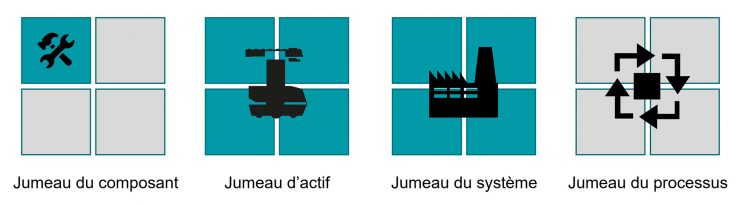
\includegraphics{images/types-de-jumeaux-numeriques.jpg}}
    \caption{Les différents types de jumeau numérique}
    {source : Jumeau numérique en logistique, KNAPP\footcite{JumeauNumeriqueLogistique2023}}
\end{figure}

\begin{itemize} 
 \item \textbf{Jumeaux de composant (component twins, ou part twins)} : Les jumeaux de composant sont la représentation numérique d'une seule pièce qui assure une fonction clé dans d'un système complet. Il peut s’agir par exemple d'un moteur dans une éolienne. 
 \item \textbf{Jumeaux d'actif (asset twins)} : Un actif est un élément individuel, souvent une machine ou un équipement, qui peut faire partie d'un système plus vaste. Un jumeau d'actifs revient à représenter la combinaison de deux composants (les actifs) ou plus qui fonctionnent ensembles. Ce type de jumeau numérique représente un seul équipement ou une machine spécifique, ou un ensemble de composants qui fonctionnent ensemble comme une unité unique. Par exemple, un jumeau d'actif pourrait représenter comment le moteur et les pales d'une éolienne travaillent ensemble pour produire de l'énergie.
 \item \textbf{Jumeau de système ou jumeau d’unité (system or unit twins)} : il s’agit de la représentation de diverses ressources dans un même système. Le jumeau numérique fournit et met en commun des informations sur l’interaction des installations et sur des améliorations possibles de la performance, par exemple de la production globale. Ce type de jumeau numérique représente un ensemble plus large et complexe de machines ou d'équipements, souvent au niveau d'une installation entière ou d'un processus global.
 \item \textbf{Jumeaux de processus (process twins)} : Les jumeaux de processus sont des représentations numériques des procédures et des flux de travail, plutôt que des représentations d’un produit physique. Ils modélisent, au sein d’un environnement numérique, comment les différents composants, équipements et unités interagissent et fonctionnent ensemble. Ils indiquent comment les système fonctionne pour créer une installation de production globale. Par exemple, un jumeau de processus peut reproduire le fonctionnement complet d'une usine de fabrication, incluant tous les composants et machines qu'elle contient. Cela permet d'analyser et d'améliorer les processus opérationnels, d'identifier les inefficacités et de tester des changements sans affecter l'environnement réel. \footcite{QuEstceQu2023}\footcite{JumeauNumeriqueLogistique2023}
\end{itemize}

Pour résumer, un jumeau numérique peut donc représenter : une seule pièce d’un produit, plusieurs pièces ou composants qui fonctionnent ensemble, un système complet, un processus.\\

Parmi ces distinctions, d’autres types de jumeaux numériques de distinguent. Ils sont quant à eux définis par le moment où ils sont créés, c'est-à-dire avant, pendant ou après la création du produit\footcite{DigitalTwin2024} \footcite{rebecchiQuEstceQue2021}.\\

\begin{itemize}
    \item \textbf{Prototype de jumeau numérique (digital Twin prototype)} : Ce type se compose des conceptions, analyses et processus nécessaires à la réalisation d'un produit physique. Utilisé avant la création du produit, il permet de tester et d'optimiser les caractéristiques du produit dans un environnement virtuel avant sa fabrication.
    \item \textbf{-	Instance de jumeau numérique (Digital Twin Instance)} : Une fois que le produit est fabriqué, ce jumeau numérique représente chaque instance individuelle du produit. Il est lié à son homologue physique pour toute la durée de vie de ce dernier, permettant de réaliser des tests sur différents scénarios d'utilisation et de surveiller la performance en temps réel.
    \item \textbf{-	Agrégat de jumeau numérique (Digital Twin Aggregate)} : Ce type regroupe les informations provenant des différentes instances de jumeaux numériques (DTI). Ces données peuvent être utilisées pour des interrogations sur le produit physique, des pronostics et des apprentissages. L'agrégat permet de déterminer les capacités globales d'un produit, d'effectuer des prévisions et d'optimiser les paramètres de fonctionnement.\\
\end{itemize}

On peut estimer que le projet C-ADER utilisera le modèle du jumeau de composant ou de pièce. En effet, les jumeaux de composant ou de pièce se concentrent sur des parties individuelles d'un système plus vaste. Justement, l’objectif pensé pour la réalisation du jumeau numérique est de rendre chaque partie de l'avion scannée (donc chaque composant unique) cliquable. Chaque partie de l'avion serait numérisée et rendue interactivement accessible, permettant aux utilisateurs d'explorer des informations détaillées sur chaque composant individuel. Cette approche correspond étroitement à la définition des jumeaux numériques de composant ou de pièce, où l'accent est mis sur la granularité des données et la possibilité d'accéder à des détails spécifiques sur les éléments constitutifs.\\

En raison de la nature statique de l'avion exposé dans un musée, les composants individuels ne subissent pas de changements dynamiques fréquents. Cette caractéristique est typique des jumeaux de composant plutôt que des jumeaux de processus ou de systèmes, qui sont davantage orientés vers la gestion et l'optimisation de processus dynamiques en temps réel.  De même, les jumeaux de systèmes ou d'unités, qui se concentrent sur l'assemblage fonctionnel de divers actifs pour améliorer les performances globales, semblent mieux adaptés à des environnements opérationnels et dynamiques. Enfin, les jumeaux de processus, qui suivent et optimisent les flux de travail dynamiques, ne s'appliquent pas directement à un avion exposé comme c'est le cas.\\

Ces différents types et approches témoignent ainsi de la grande flexibilité de l'outil, ce qui contribue à expliquer la très large popularité de cet outil dans des cadres assez variés.\\

